\chapter{Evaluation}
This chapter presents the results of the evaluation of our approach. The experiments have been conducted based on several test parameters and their combinations and we will be analyzing the baseline parameter sets as well as key combinations. 

We evaluate based on the path length, capacity range, packet size, number of packets. For the better insight we also apply artificial packet loss and icmp rate limit. 
The tests are conducted on the empty network as well as with significant amount of cross-traffic load.

The following parameters must be passed to the program via the config file:
\begin{itemize}
	\item \texttt{topo\textunderscore size} - The number of routers between the source host and the destination host.
	\item \texttt{capacity\textunderscore range} - The range of numbers from which a capacity for each link will be generated
	\item \texttt{packet\textunderscore size} - The size of each packet (in bytes) that will be sent from the source host to the destination.
	\item \texttt{packets\textunderscore per\textunderscore hop} - The amount of packets that will be targeted at each hop
	\item \texttt{icmp\textunderscore ratelimit} - The artificial ICMP rate limit that will be assigned to each router. The default value is 0.
	\item \texttt{packet\textunderscore loss} - The artificial packet loss that will be assigned to each router. The default value is 0.
	\item \texttt{cross\textunderscore traffic} - The coefficient of the cross traffic load. The Optimal value is recommended to be assigned from 0 to 1.0, the value of 0 meaning an empty network without any cross traffic. 
\end{itemize}


\section{Test Environment and Setup}
For the testing purposes we decided to build a virtual network using the network emulator - Mininet\cite{mnHome}. It provides the necessary tools to create an artificial network and has a very handy Python API that enables us to build custom topologies.


The figure below represents the template of the network that we have used in our experiments. It consists of the source and destination hosts, the top and bottom hosts and routers that connects them with each other. \\

\begin{figure}[htp]
 \centering
	 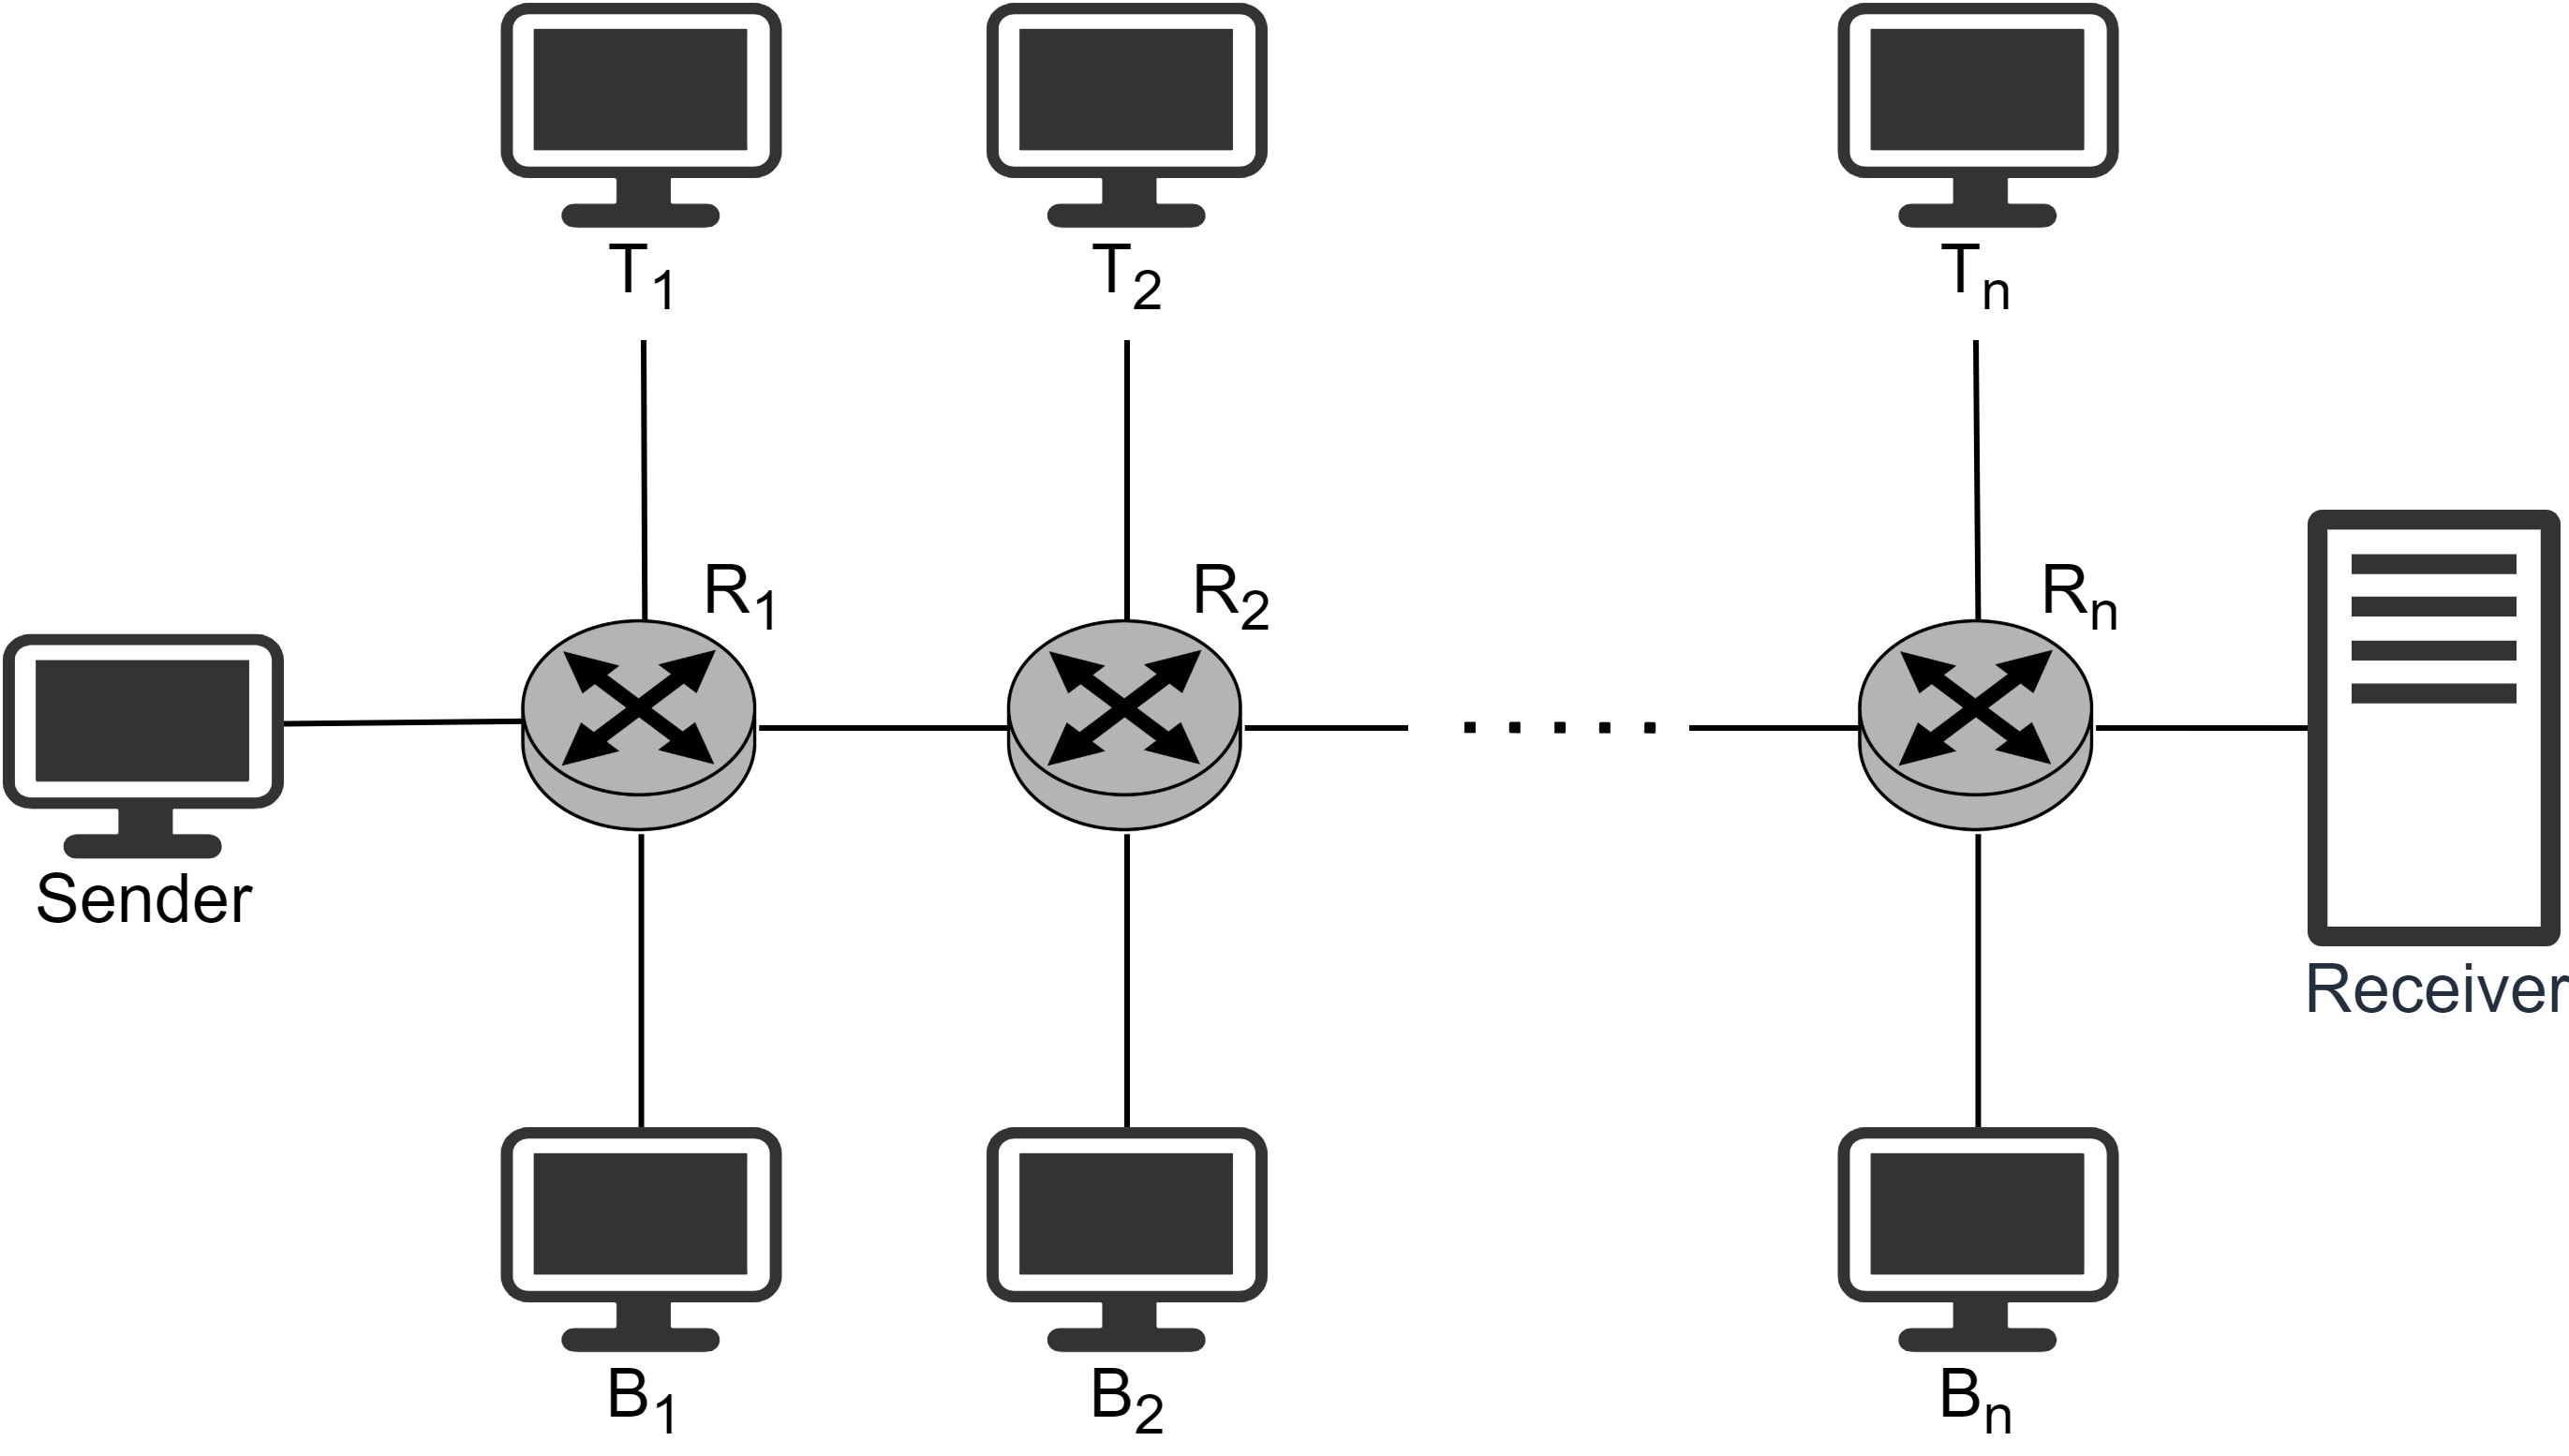
\includegraphics[width=\textwidth]{topology}
 \caption{The template network topology}
 \label{topology}

\end{figure}

As a reader can see from the Figure \ref{topology}, the main hosts (sender and receiver) are connected with a sequence of \texttt{n} routers, each consisting of four interfaces and each having its own subnetwork. The number of routers and, therefore, the number of top and bottom hosts is dynamic and configurable. The routes from and to all hosts are statically configured.

The measurements are conducted based on the main path, which is the one that connects the sender to the receiver. Top and bottom hosts are used for generating cross-traffic in later experiments. Cross-traffic interferes with the main flow of packets and has a significant influence on the accuracy of capacity estimations.  

The measuring node is "Sender", as using our tool only makes sense if the measuring node is the one that generates the traffic. All the necessary traffic is captured at this node with the \texttt{tcpdump} command and subsequently analyzed in order to deliver the result.

Finally, it is also important to mention that Mininet has certain limitations, namely, it is limited with the computational power of the machine it runs on. Therefore we have decided to execute the estimation experiments on the testbed of the chair.
Each set of parameters have been tested 20 times to ensure the reliable results.

\section{Evaluation in Empty Network}
We decided to divide our evaluation into two parts: Measurements on empty network and on relatively overloaded network where the flow of our measurements is interfered by cross-traffic. 

\subsection{Path Length}
The first parameter to be discussed is the path length from the source host to the sink, i.e. number of hops on the path. In order to analyze the impact that a path length can have on the measurement accuracy, we have to execute the test runs on different values of the given parameter. \\
We decided to conduct measurements on arbitrary numbers of routers, namely 3, 8, 20 and 32. They paint a good picture of how our estimation tool reacts on networks with different sizes. 

\begin{figure}[H]%[!tbp]
  \centering
  \begin{minipage}[b]{0.45\textwidth}
    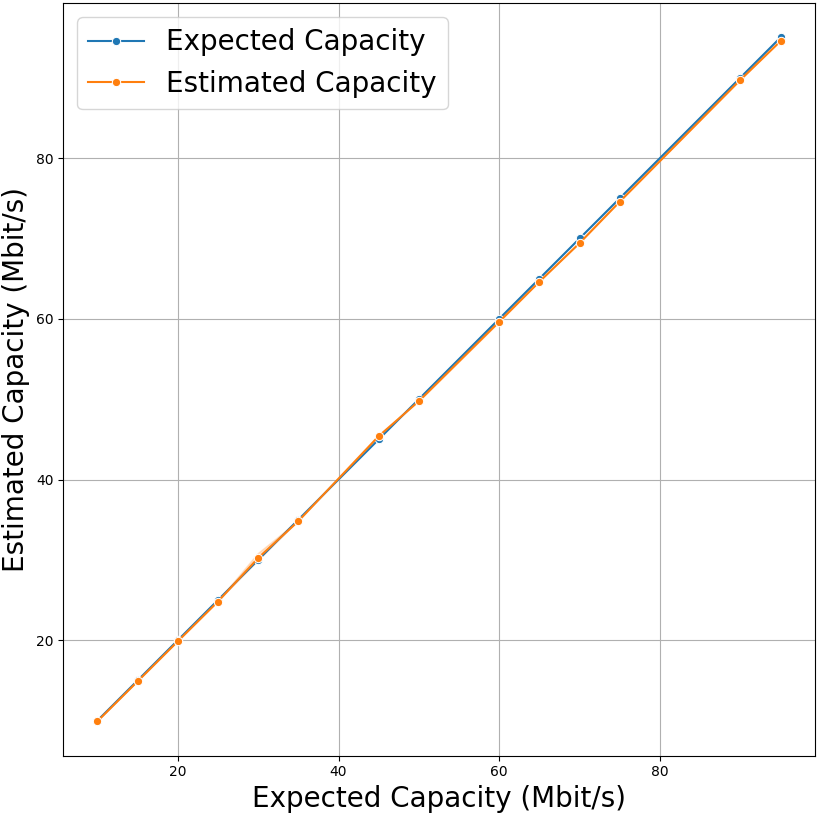
\includegraphics[width=\textwidth]{topo_size/topo_size_3}
    \caption{Path length: 3 Routers}
  \end{minipage}
  \hfill
  \begin{minipage}[b]{0.45\textwidth}
    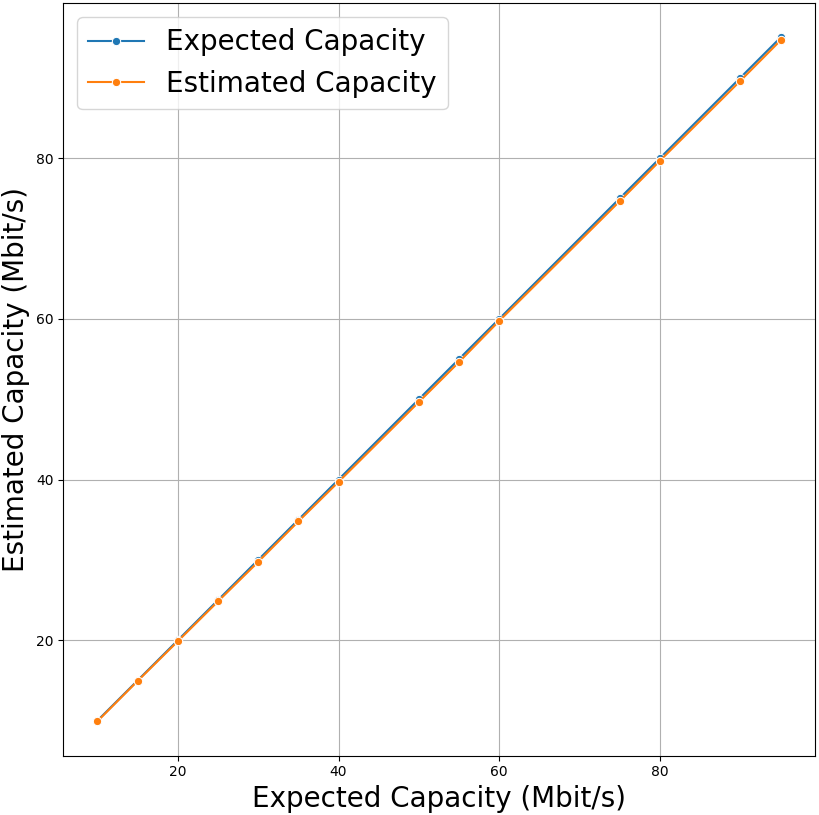
\includegraphics[width=\textwidth]{topo_size/topo_size_32}
    \caption{Path length: 32 Routers}
  \end{minipage}
\end{figure}


\begin{table}[h!]
\centering
 \begin{tabular}{||c ||c c c c||} 
 \hline
 Path Length & Standard Deviation & Average & Min Error & Max Error \\ [0.5ex] 
 \hline\hline
 3 & 3.74\% & 4.78\% & 1.78\% & 19.18\% \\ 
 8 & 3.45\% & 4.94\% & 0.4\% & 20.17\% \\
 20 & 2.93\% & 4.17\% & 0.64\% & 28.79\% \\
 32 & 2.45\% & 4.21\% & 0.11\% & 20.23\% \\
 63 & 4.06\% & 5.02\% & 0.02\% & 24.97\% \\ [1ex] 
 \hline
 \end{tabular}
 \caption{Error Statistics of paths with different lengths}

\end{table}


\subsection*{Conclusion}
We can conclude that the path length doesn't affect the accuracy of the estimation tool. After testing the path length we decided to take 8 routers as a default path length for the posterior estimations
\\
Notes\\
gets weirdly accurate around 35-40\\
description of table is required\\

\subsection{Packet Size}
One of the key parameters in our evaluation is the packet size. 
As the packet size along with the amount of packets that have to be injected into the network can be the cause of the network overload, we have to find an optimal amount of intrusion so that we don't have to sacrifice the accuracy. 

Based on the test results we were able to observe that the optimal packet size depends on the capacity range of the network. 

\subsection*{Estimation Error}

\subsection*{Conclusion}

\subsection{Train Length}

\subsection*{Conclusion}


\subsection{Optimal Intrusion}

\subsection{Capacity Range}
One of the most important parameters is the capacity range of the links that we conduct our measurements on. After testing the tool on several different networks with varying capacity ranges, such as [10, 100], as well as [500, 600] and [1000, ..] it appears that our methodology has a significant limitation when measuring the networks that contain links with relatively high capacities. 

\subsection*{Conclusion}
In conclusion, we can deduce that the accuracy of the tool greatly depends on the capacity range. We can argue that on an empty network the accuracy is good for the paths that have the capacity value up to XXX Mbits. We expect that the tool accuracy when measuring the links with capacities over XXX will be less reliable during cross-traffic. In other words the accuracy threshold will be lower. We will discuss this in the section about cross-traffic.


\subsection{Packet Loss}

\subsection{ICMP Rate Limiting}
Provide the information about icmp rate limiting and then how it affects your experiment results

\subsection{Summary}


\section{Evaluation during Cross-Traffic}
We have conducted the previous experiments on empty networks without any cross-traffic. However this is not the case in the real Internet that we use on daily basis. 
Cross traffic seems to affect the test results significantly. 
What does 1.0 mean?

\subsection{Path Length}

\subsection{Packet Size}

\subsection{Train Length}

\subsection{Optimal Intrusion during Cross-Traffic}

\subsection{Capacity Range}

\subsection{Packet Loss}

\subsection{ICMP Rate Limiting}

\subsection{Combination of Cross-Traffic, Artificial Packet Loss and ICMP Rate Limiting}

\subsection{Summary}


\section{Data Replication}
One option to try to see if it can help
